\def\lecturenumber{10}
\documentclass[11pt,a4paper]{article}
\usepackage[T1]{fontenc}
\usepackage[utf8]{inputenc}
\usepackage{lmodern}
\usepackage[margin=19mm,top=21mm,bottom=21mm,headheight=15pt]{geometry}
\usepackage{amsmath,amssymb,booktabs,array,graphicx,microtype}
\usepackage[dvipsnames]{xcolor}
\usepackage{enumitem,fancyhdr,listings,tcolorbox}
\usepackage[colorlinks=true,linkcolor=MidnightBlue,urlcolor=MidnightBlue]{hyperref}
\definecolor{courseblue}{HTML}{164B69}
\definecolor{pale}{HTML}{F0F5F7}
\pagestyle{fancy}
\fancyhf{}
\fancyhead[L]{\small\sffamily\color{courseblue}VALIDATED COMPUTING}
\fancyhead[R]{\small\sffamily Lecture \lecturenumber}
\fancyfoot[L]{\footnotesize Expanded lecture notes \textbullet\ October 2026}
\fancyfoot[R]{\footnotesize\thepage\ / 6}
\renewcommand{\headrulewidth}{0.4pt}
\setlength{\parindent}{0pt}
\setlength{\parskip}{5.5pt plus 1pt}
\setlength{\emergencystretch}{1.5em}
\setlist[itemize]{leftmargin=1.5em,itemsep=3pt,topsep=3pt}
\setlist[enumerate]{leftmargin=1.7em,itemsep=5pt,topsep=4pt}
\lstset{language=Python,basicstyle=\small\ttfamily,keywordstyle=\color{courseblue}\bfseries,
 commentstyle=\color{OliveGreen},stringstyle=\color{BrickRed},showstringspaces=false,
 columns=fullflexible,keepspaces=true,frame=single,rulecolor=\color{black!18},
 backgroundcolor=\color{black!2},aboveskip=6pt,belowskip=6pt,breaklines=true,
 xleftmargin=5pt,xrightmargin=5pt,framesep=5pt}
\newcommand{\R}{\mathbb R}
\newcommand{\fl}{\operatorname{fl}}
\newcommand{\abs}[1]{\left|#1\right|}
\newcommand{\heading}[2]{\section*{\color{courseblue}#1}\vspace{-4pt}{\small\sffamily\color{black!65}#2}\par\vspace{3pt}}
\newcommand{\opening}[2]{{\Large\sffamily\bfseries\color{courseblue}Lecture \lecturenumber\quad #1\par}\vspace{5pt}{\small #2}\par}
\newtcolorbox{question}[1]{colback=pale,colframe=courseblue!55,boxrule=0.4pt,
 arc=1mm,left=7pt,right=7pt,top=4pt,bottom=4pt,title={#1},fonttitle=\bfseries\small,
 coltitle=courseblue,colbacktitle=pale}
\newcommand{\reading}[1]{{\footnotesize\textbf{Reading and notebook.} #1\par}}
\hypersetup{pdfauthor={Validated Computing course},pdfsubject={Expanded introductory lecture notes with questions and exercises}}

\hypersetup{pdftitle={Lecture 10: Certifying a root of a nonlinear system}}
\begin{document}
\opening{Certifying a root of a nonlinear system}{Prerequisites: Lectures 08--09; matrix multiplication and elementary derivatives.\newline
Goal: certify one root in a specified box using a fixed-point enclosure and an explicit contraction bound.}
\heading{1. From an approximate intersection to a box certificate}{0--13 minutes: the problem, the data, and the local claim}
Consider the system
\[
 f(x,y)=\begin{pmatrix}x^2+y^2-1\\x-y\end{pmatrix}=0.
\]
We seek intersections of the unit circle with the line $x=y$. Substitution
gives the two exact solutions $(1/\sqrt2,1/\sqrt2)$ and
$(-1/\sqrt2,-1/\sqrt2)$. This algebra provides an independent reference.
Our computational task is to certify exactly one root in the positive box
\[
               X=[7/10,18/25]\times[7/10,18/25]=[0.70,0.72]^2.
\]
A numerical solver could propose such a box. Its proposal is useful even
when its iteration history is not a proof. The certificate will depend on
explicit bounds on this box, not on a claim that the solver converged.

A box is a Cartesian product of intervals. The midpoint here is the exact
vector $m=(71/100,71/100)^T$. A vector belongs to the box when each
coordinate belongs to its interval. A box $Y$ lies strictly inside $X$ when
each lower endpoint of $Y$ is strictly above the corresponding lower
endpoint of $X$, and each upper endpoint is strictly below its counterpart.

The Jacobian is the matrix of partial derivatives,
\[
 J_f(x,y)=\begin{pmatrix}2x&2y\\1&-1\end{pmatrix}.
\]
Lecture 08's interval automatic differentiation can enclose its entries.
Here we can also derive the interval matrix directly:
\[
 J(X)=\begin{pmatrix}[7/5,36/25]&[7/5,36/25]\\1&-1\end{pmatrix}.
\]
Constants in this display mean point intervals. Every real Jacobian on $X$
belongs entry by entry to $J(X)$. Some combinations of interval entries
may not occur at the same point; interval matrix operations allow that
overestimation while preserving inclusion.

\begin{question}{State the scope before calculating}
If we certify exactly one root in this box, what has been proved about the
negative solution? Would a tiny residual at $m$ alone prove uniqueness?
List the distinction between a candidate point, a candidate box, and a certificate.
\end{question}

Throughout this lecture assume $f$ is continuously differentiable on a
neighborhood of a closed box with positive side widths. The Jacobian
enclosure must hold throughout that box. Matrix entries and intermediate
results must use exact or inclusion-preserving arithmetic. A matrix of
derivatives evaluated only at $m$ does not supply this whole-box premise.

\newpage
\heading{2. Turn the root equation into a fixed-point equation}{13--30 minutes: derive the Krawczyk enclosure}
Choose a fixed nonsingular real matrix $R$, usually close to the inverse
Jacobian at $m$, and define
\[
                         T(z)=z-Rf(z).
\]
Every root is a fixed point of $T$. Conversely, $T(z)=z$ implies
$Rf(z)=0$, hence $f(z)=0$ because $R$ is nonsingular. The matrix is called
a preconditioner: a good choice makes $T'(z)=I-RJ_f(z)$ small on the box.
It is a point matrix, not an interval inverse that changes from point to point.

\textbf{The vector mean-value argument.} A box is convex, so the segment
from $m$ to any $z\in X$ stays in $X$. Applying the fundamental theorem of
calculus along this segment gives
\[
 f(z)-f(m)=A_z(z-m),\qquad
 A_z=\int_0^1 J_f\bigl(m+t(z-m)\bigr)\,dt.
\]
Each entry of $A_z$ lies in its corresponding interval in $J(X)$.
We do not need, and generally cannot assert, a single point $\xi$ whose
Jacobian equals this entire average matrix. The integral avoids that
incorrect extension of the scalar mean value theorem.

Substitution into $T$ yields
\[
 T(z)=m-Rf(m)+(I-RA_z)(z-m).
\]
Let $C$ be a valid vector enclosure of $f(m)$, and evaluate the interval
matrix $E=I-RJ(X)$. Then
\[
                  T(X)\subseteq K(X):=m-RC+E(X-m).
\]
This is the Krawczyk enclosure used here. Matrix multiplication consists of
ordinary row-by-column sums with interval products. Each operation may
widen the result, but every actual value $T(z)$ remains enclosed.

\textbf{Immediate root retention.} If $r\in X$ is a root, then
$r=T(r)\in K(X)$. Consequently every root in $X$ lies in $X\cap K(X)$.
If the boxes are disjoint, there is no root in $X$. Disjointness in just one
coordinate is enough: no vector can belong to both boxes in that case.
A nonempty intersection alone still proves no existence.

\begin{question}{Inspect the role of each object}
Identify which quantities are fixed point data and which are interval
enclosures. Why does replacing $J(X)$ by $J_f(m)$ invalidate the argument
in general? What would happen to the root--fixed-point equivalence if $R=0$?
\end{question}

The enclosure is useful when $R$ approximately cancels the Jacobian,
leaving a small remainder $E$. An approximate inverse can therefore be an
excellent proposal. Its quality will be measured by rigorous bounds on
$E$ and $K(X)$, rather than assumed from the inversion algorithm's name.

\newpage
\heading{3. Check both invariance and contraction}{30--46 minutes: a sufficient theorem with a short proof}
For vectors define $\|v\|_\infty=\max_j|v_j|$. For a point matrix $A$,
the corresponding norm is $\|A\|_\infty=\max_i\sum_j|A_{ij}|$.
If $E_{ij}=[\underline e_{ij},\overline e_{ij}]$, a valid upper bound for
the norm of every represented matrix is
\[
 q=\max_i\sum_j\max\bigl(|\underline e_{ij}|,|\overline e_{ij}|\bigr).
\]
The row-sum formula follows by bounding
$|(Av)_i|\le\sum_j|A_{ij}|\,\|v\|_\infty$. With machine endpoints, compute
the bound upwards. An ordinary rounded-down row sum could falsely pass $q<1$.

Our sufficient success test requires both
\[
                   K(X)\subset\operatorname{int}(X),\qquad q<1.
\]
The first condition implies $T(X)\subseteq X$. The second, together with
the derivative enclosure and a segment integral, gives
$\|T(u)-T(v)\|_\infty\le q\|u-v\|_\infty$ for every $u,v\in X$.
Thus $T$ maps the closed box into itself and is a contraction there.

\textbf{Why a fixed point exists.} Start with any $z_0\in X$ and set
$z_{n+1}=T(z_n)$. All iterates stay in $X$. Successive distances satisfy
$\|z_{n+1}-z_n\|_\infty\le q^n\|z_1-z_0\|_\infty$. For $k\ge1$,
\[
 \|z_{n+k}-z_n\|_\infty
 \le\frac{q^n}{1-q}\,\|z_1-z_0\|_\infty.
\]
This tends to zero, so the iterates are Cauchy. The closed box contains
their limit, and continuity of $T$ makes that limit a fixed point. If $u$
and $v$ were two fixed points, their distance would be at most $q$ times
itself, forcing $u=v$. This is the contraction mapping theorem in the
specific form needed here. Nonsingular $R$ turns the unique fixed point
into the unique root of $f$ in $X$.

\begin{question}{Why two separate inequalities?}
The map $T(t)=t/2+2$ has derivative norm $1/2$ on $[-1,1]$. Where is its
fixed point? Which hypothesis fails on this interval? Explain why a small
derivative norm alone cannot certify a root inside the proposed domain.
\end{question}

The computational outcomes are now precise. A disjoint Krawczyk image
proves exclusion. Strict inclusion plus $q<1$ proves exactly one root.
Otherwise this test is inconclusive. Strictness and the row-sum test make
our teaching criterion conservative: failure does not imply that no root
exists, that several roots exist, or that stronger verification methods fail.

\newpage
\heading{4. Work one certificate all the way to exact fractions}{46--61 minutes: circle, line, and the final box}
For the box on page 1, the midpoint Jacobian and its exact inverse are
\[
 J_f(m)=\begin{pmatrix}71/50&71/50\\1&-1\end{pmatrix},\qquad
 R=\begin{pmatrix}25/71&1/2\\25/71&-1/2\end{pmatrix}.
\]
The determinant of $R$ is $-25/71\ne0$. At the midpoint,
$f(m)=(41/5000,0)^T$. Both coordinates of the corrected centre are
\[
             s=\frac{71}{100}-\frac{25}{71}\frac{41}{5000}
               =\frac{10041}{14200}.
\]
This point resembles a Newton update, but is not yet a root enclosure.
The remainder matrix supplies the necessary spread around it.

For example, its first row is
\[
 E_{11}=\frac12-\frac{50}{71}X_1,
 \qquad E_{12}=\frac12-\frac{50}{71}X_2.
\]
Both intervals are $[-1/142,1/142]$. The second row gives the same
intervals. Therefore $q=2/142=1/71<1$. Each coordinate of $X-m$
is $[-1/100,1/100]$, and summing the two interval products gives
$[-1/7100,1/7100]$ in each coordinate. Consequently
\[
 K(X)=\left[\frac{10039}{14200},\frac{10043}{14200}\right]^2
                 \subset\operatorname{int}([0.70,0.72]^2).
\]
All of these are exact rational computations. Both theorem conditions
hold, so there is exactly one root in the original box and it lies in this
smaller box. The enclosure may include points off the line and off the
circle; enclosing a root does not make every enclosed point a solution.

\begin{center}
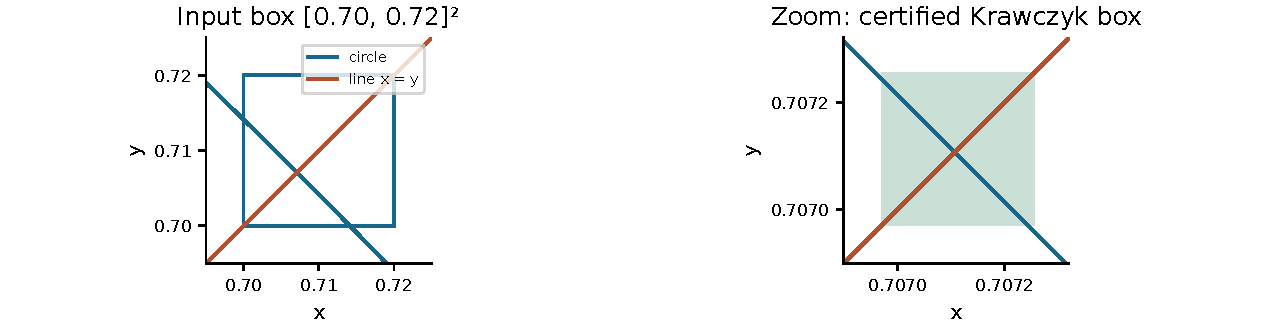
\includegraphics[width=0.9\linewidth]{figures/system_certificate.pdf}
\end{center}

\begin{question}{Check a row of the certificate independently}
Derive $E_{21}$ and $E_{22}$ using ordinary row-by-column multiplication.
Verify the strict lower and upper endpoint inequalities for $K(X)$.
Which step proves existence, and which expression specifies the root's location?
\end{question}

The exact solution provides a separate check: each positive coordinate
interval $[l,u]$ satisfies $2l^2<1<2u^2$. This is a useful diagnostic.
The general certificate, however, does not rely on knowing the answer in advance.

\newpage
\heading{5. Readable checks and an approximate inverse proposal}{61--77 minutes: verify the certificate, not the proposal's pedigree}
The following standalone code checks the exact quantities just derived.
The common endpoint radius for $E$ comes from the interval matrix
calculation on page 4; it is not inferred by sampling Jacobians.
\begin{lstlisting}
from fractions import Fraction

left, right = Fraction("0.70"), Fraction("0.72")
center = (left + right) / 2
radius = (right - left) / 2
R = [[Fraction(25, 71), Fraction(1, 2)],
     [Fraction(25, 71), Fraction(-1, 2)]]
determinant = R[0][0]*R[1][1] - R[0][1]*R[1][0]
assert determinant != 0
residual = 2*center*center - 1
corrected_center = center - R[0][0]*residual
entry_radius = Fraction(1, 142)
q = 2 * entry_radius
spread = 2 * entry_radius * radius
lower = corrected_center - spread
upper = corrected_center + spread
assert (lower, upper) == (Fraction(10039, 14200),
                          Fraction(10043, 14200))
assert left < lower and upper < right and q < 1
assert 2*lower*lower < 1 < 2*upper*upper
\end{lstlisting}

For a different system, a matrix routine such as \texttt{numpy.linalg.inv}
may propose $R$. Interpret each stored float entry as an exact real number,
for example using \texttt{Fraction.from\_float}. Then verify nonsingularity
and recompute $E$, $K$, and $q$ rigorously. The theorem never required
$R=J_f(m)^{-1}$ exactly. A slightly imperfect inverse merely changes the
matrix being checked and often still succeeds.

Increasing the working precision when constructing enclosures may reduce
rounding width. It cannot remove Jacobian variation across a wide box or
turn two actual roots in that box into one. A failed test may instead need
a smaller box, a better candidate centre, or a different preconditioner.
Every changed box or matrix requires a fresh check of the premises.

\begin{question}{What must be saved to review this result?}
List the input box, exact centre, point matrix, midpoint residual enclosure,
Jacobian enclosure, remainder matrix, Krawczyk image, and norm bound.
Which data would a reviewer be missing if only the final status were printed?
\end{question}

Notebook 10 computes all matrix entries with short loops and records these
objects. Its successful local result does not implement an exhaustive
two-dimensional search. Extending the root-search invariant of Lecture 09
to boxes is possible, but requires decisions for every region and explicit
handling of unresolved boxes.

\newpage
\heading{6. A zero residual can coexist with two nearby roots}{77--90 minutes: a failure case and selected exercises}
Let $\varepsilon=10^{-6}$ and consider
\[
 g(x,y)=\bigl(x+y,\ x+(1+\varepsilon)y+x^2\bigr).
\]
The first equation gives $y=-x$; the second then becomes
$x(x-\varepsilon)=0$. Thus both $(0,0)$ and
$(\varepsilon,-\varepsilon)$ are roots. The box $[-1/100,1/100]^2$
contains both. Its midpoint residual is exactly zero, but no valid theorem
can certify uniqueness on that box. The midpoint Jacobian has determinant
$\varepsilon$; its large inverse amplifies variation. With its exact inverse,
our row-sum bound is $q=20000$, so the sufficient test fails honestly.

\begin{enumerate}
\item \textbf{Read a norm bound.} Suppose the remainder matrix is
$E=\left(\begin{smallmatrix}[-1/10,1/5]&[0,1/10]\\{}[-1/4,1/4]&[-1/8,1/8]\end{smallmatrix}\right)$.
Compute $q$. Does that number alone prove a root exists in a given box?
State the missing geometric and algebraic conditions.

\item \textbf{Reject a false equivalence.} Set $R=0$ in $T(z)=z-Rf(z)$.
Show that every point is fixed, regardless of $f$. Compute $E$ and $q$.
Which part of the proof on page 2 fails? Why should the implementation
check nonsingularity rather than rely on the name ``inverse''?

\item \textbf{Reflect the successful box.} Replace the positive box by
$[-0.72,-0.70]^2$. Derive a suitable midpoint inverse and the reflected
root enclosure. What do the two local certificates say together? What
separate argument would justify that no roots exist elsewhere?

\item \textbf{Explain the failed certificate.} Verify both roots of $g$
by exact substitution. Derive the midpoint Jacobian and its determinant.
Why cannot extra precision rescue a uniqueness claim on the stated wide
box? What would need to change before trying to isolate the origin alone?
\end{enumerate}

\textbf{Selected checks.} Exercise 1: the row bounds are $3/10$ and
$3/8$, so $q=3/8$; also check $K(X)\subset\operatorname{int}(X)$,
smoothness, valid enclosures, and nonsingular $R$. Exercise 2 gives $E=I$
and $q=1$. Exercise 3 uses
$R=\left(\begin{smallmatrix}-25/71&1/2\\-25/71&-1/2\end{smallmatrix}\right)$
and gives $[-10043/14200,-10039/14200]^2$ with $q=1/71$.
Substituting $x=y$ into the circle equation supplies the separate global
argument in this example. Exercise 4: $J_g(0,0)=
\left(\begin{smallmatrix}1&1\\1&1+\varepsilon\end{smallmatrix}\right)$.
A box isolating the origin must exclude the second root and pass fresh checks.

\begin{question}{Exit ticket: state exactly what succeeded}
Give the meaning of \texttt{unique\_root}, \texttt{excluded}, and
\texttt{inconclusive}, each with its domain. Explain why neither a zero
residual nor a failed sufficient test establishes the number of roots by itself.
\end{question}

\reading{Companion: \texttt{notebooks/10\_nonlinear\_systems.ipynb} and Lab 10.
Tucker (2011), \S5.1.5 and Appendix A.4. Instructor background:
\href{https://www.tuhh.de/ti3/rump/intlab/ActaNumerica2010.pdf}{Rump, \emph{Verification methods} (2010), \S13}.
Our explicit contraction criterion is a conservative teaching variant.}
\end{document}
